\documentclass[a4paper,12pt]{article}
\usepackage{color}
\usepackage{amsmath} % do fancy math
\usepackage{mathtools}
\usepackage{amsfonts}
\usepackage{bm}
\usepackage{amsthm} % math theorem proof etc
\usepackage{graphicx} % import images
\usepackage{tikz} % draw images with latex
%\usetikzlibrary{arrows,decorations.pathmorphing,backgrounds,positioning,fit,petri}
\usepackage{pgf} % go with tikz
\usepackage{subfigure}
\usepackage{caption}
%\usepackage{subcaption}
\usepackage{multirow}
\usepackage{algorithm}
\usepackage{algorithmic}
\usepackage{epstopdf}
\usepackage[round]{natbib}
\usepackage{setspace}
\usepackage[top=30mm, bottom=30mm, left=35mm,right=30mm]{geometry}
\newcommand{\ud}{\,\mathrm{d}}
\newcommand{\vx}{\mathbf{x}}
\newtheorem{defi}{Definition}[section]
\newtheorem{theorem}{Theorem}[section]
\newtheorem{lemma}[theorem]{Lemma}
%------------Y(^_^) I'm the happy separation line (^_^)Y-------------%


%------------Y(^_^) I'm the toolbox for lazybones (^_^)Y-------------%
% Maths
% \begin{equation*}
%
% \end{equation*}
% \mathcal{}
% \!  \,  \:  \;

% Graph
% \begin{figure}[htbp]
% \begin{center}
% \includegraphics[scale=1.1,trim=2cm 0cm 0cm 2cm]{name.pdf}
% \end{center}
% \caption[short]{long}
% \label{fig:3.2}
% \end{figure}

% Fonts
% \textbf{} \textsf{} \textit{} \textt{}

% Paragraph
% \onehalfspacing  \doublespacing
% setlength{\parindent}{0in}

% title
% \title{}
% \author{Zhe Sha}
% \date{1-Jan-1111}
% \maketitle

%------------Y(^_^) I'm the toolbox for lazybones (^_^)Y-------------%
\begin{document}

\title{Test INLA with Experiment 1}
\author{Zhe Sha}
\maketitle

\onehalfspacing
\numberwithin{equation}{section}
%------------Y(^_^) I'm the happy separation line (^_^)Y-------------%
In this report we test the INLA package by using the setting of \emph{Experiment 1a}.

\section{Introduction}
1. setting of Experiment 1a

\section{Priors for the hyper parameters }
2. Transformation of the hyper parameter and choosing the prior

\section{Test error size}
3. Test the "Principle of stable inference" theorem (cite result and paper)
\subsection{Change error size of a single point}
 Compare the effect of error size using a single isolated point.
 
 \begin{figure}[htbp]
 \begin{center}
 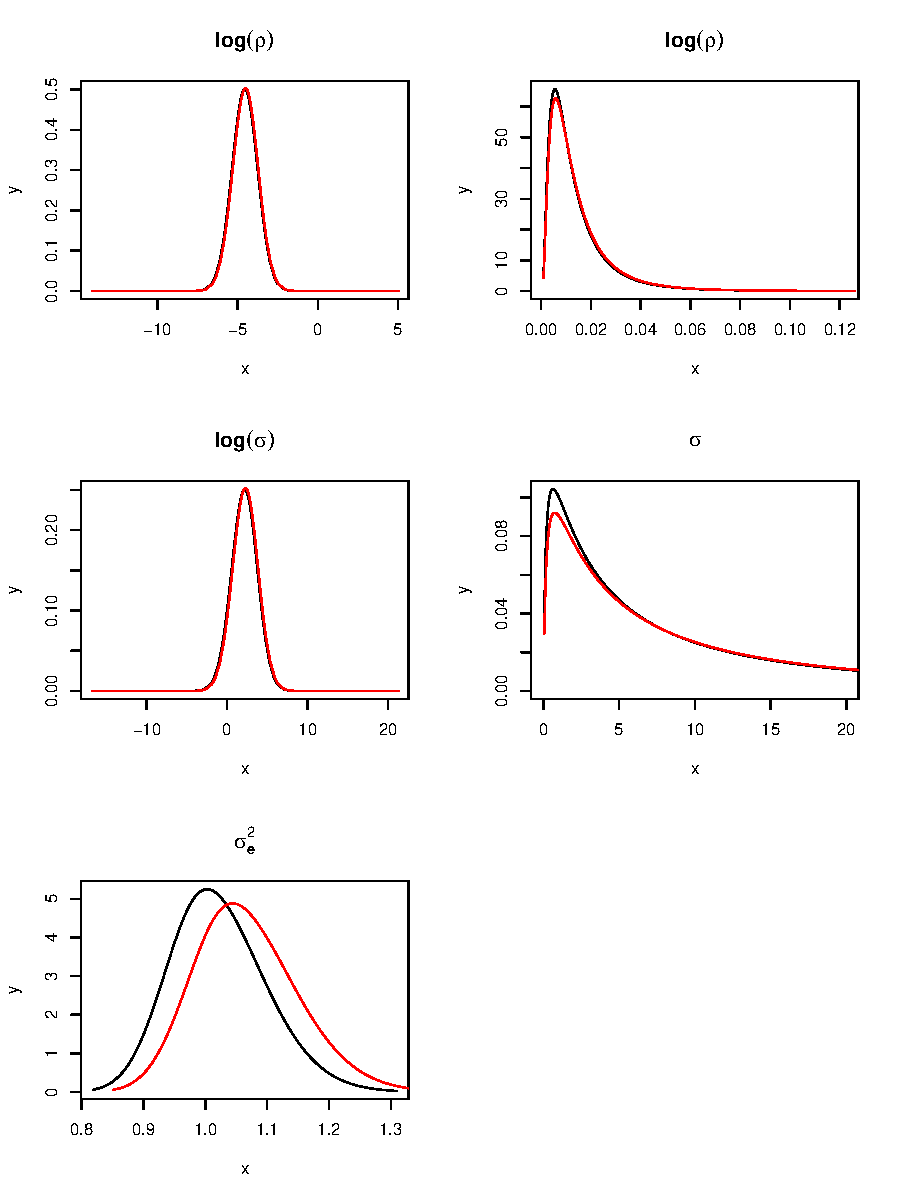
\includegraphics[scale=0.8]{fig/PointErr_hyperpar.pdf}
 \end{center}
 \caption[Posteriors of hyper parameters]{Posteriors of the hyper parameters using different error size for a selected point.}
 \label{fig:5}
 \end{figure}
 
 \begin{figure}[htbp]
 \begin{center}
 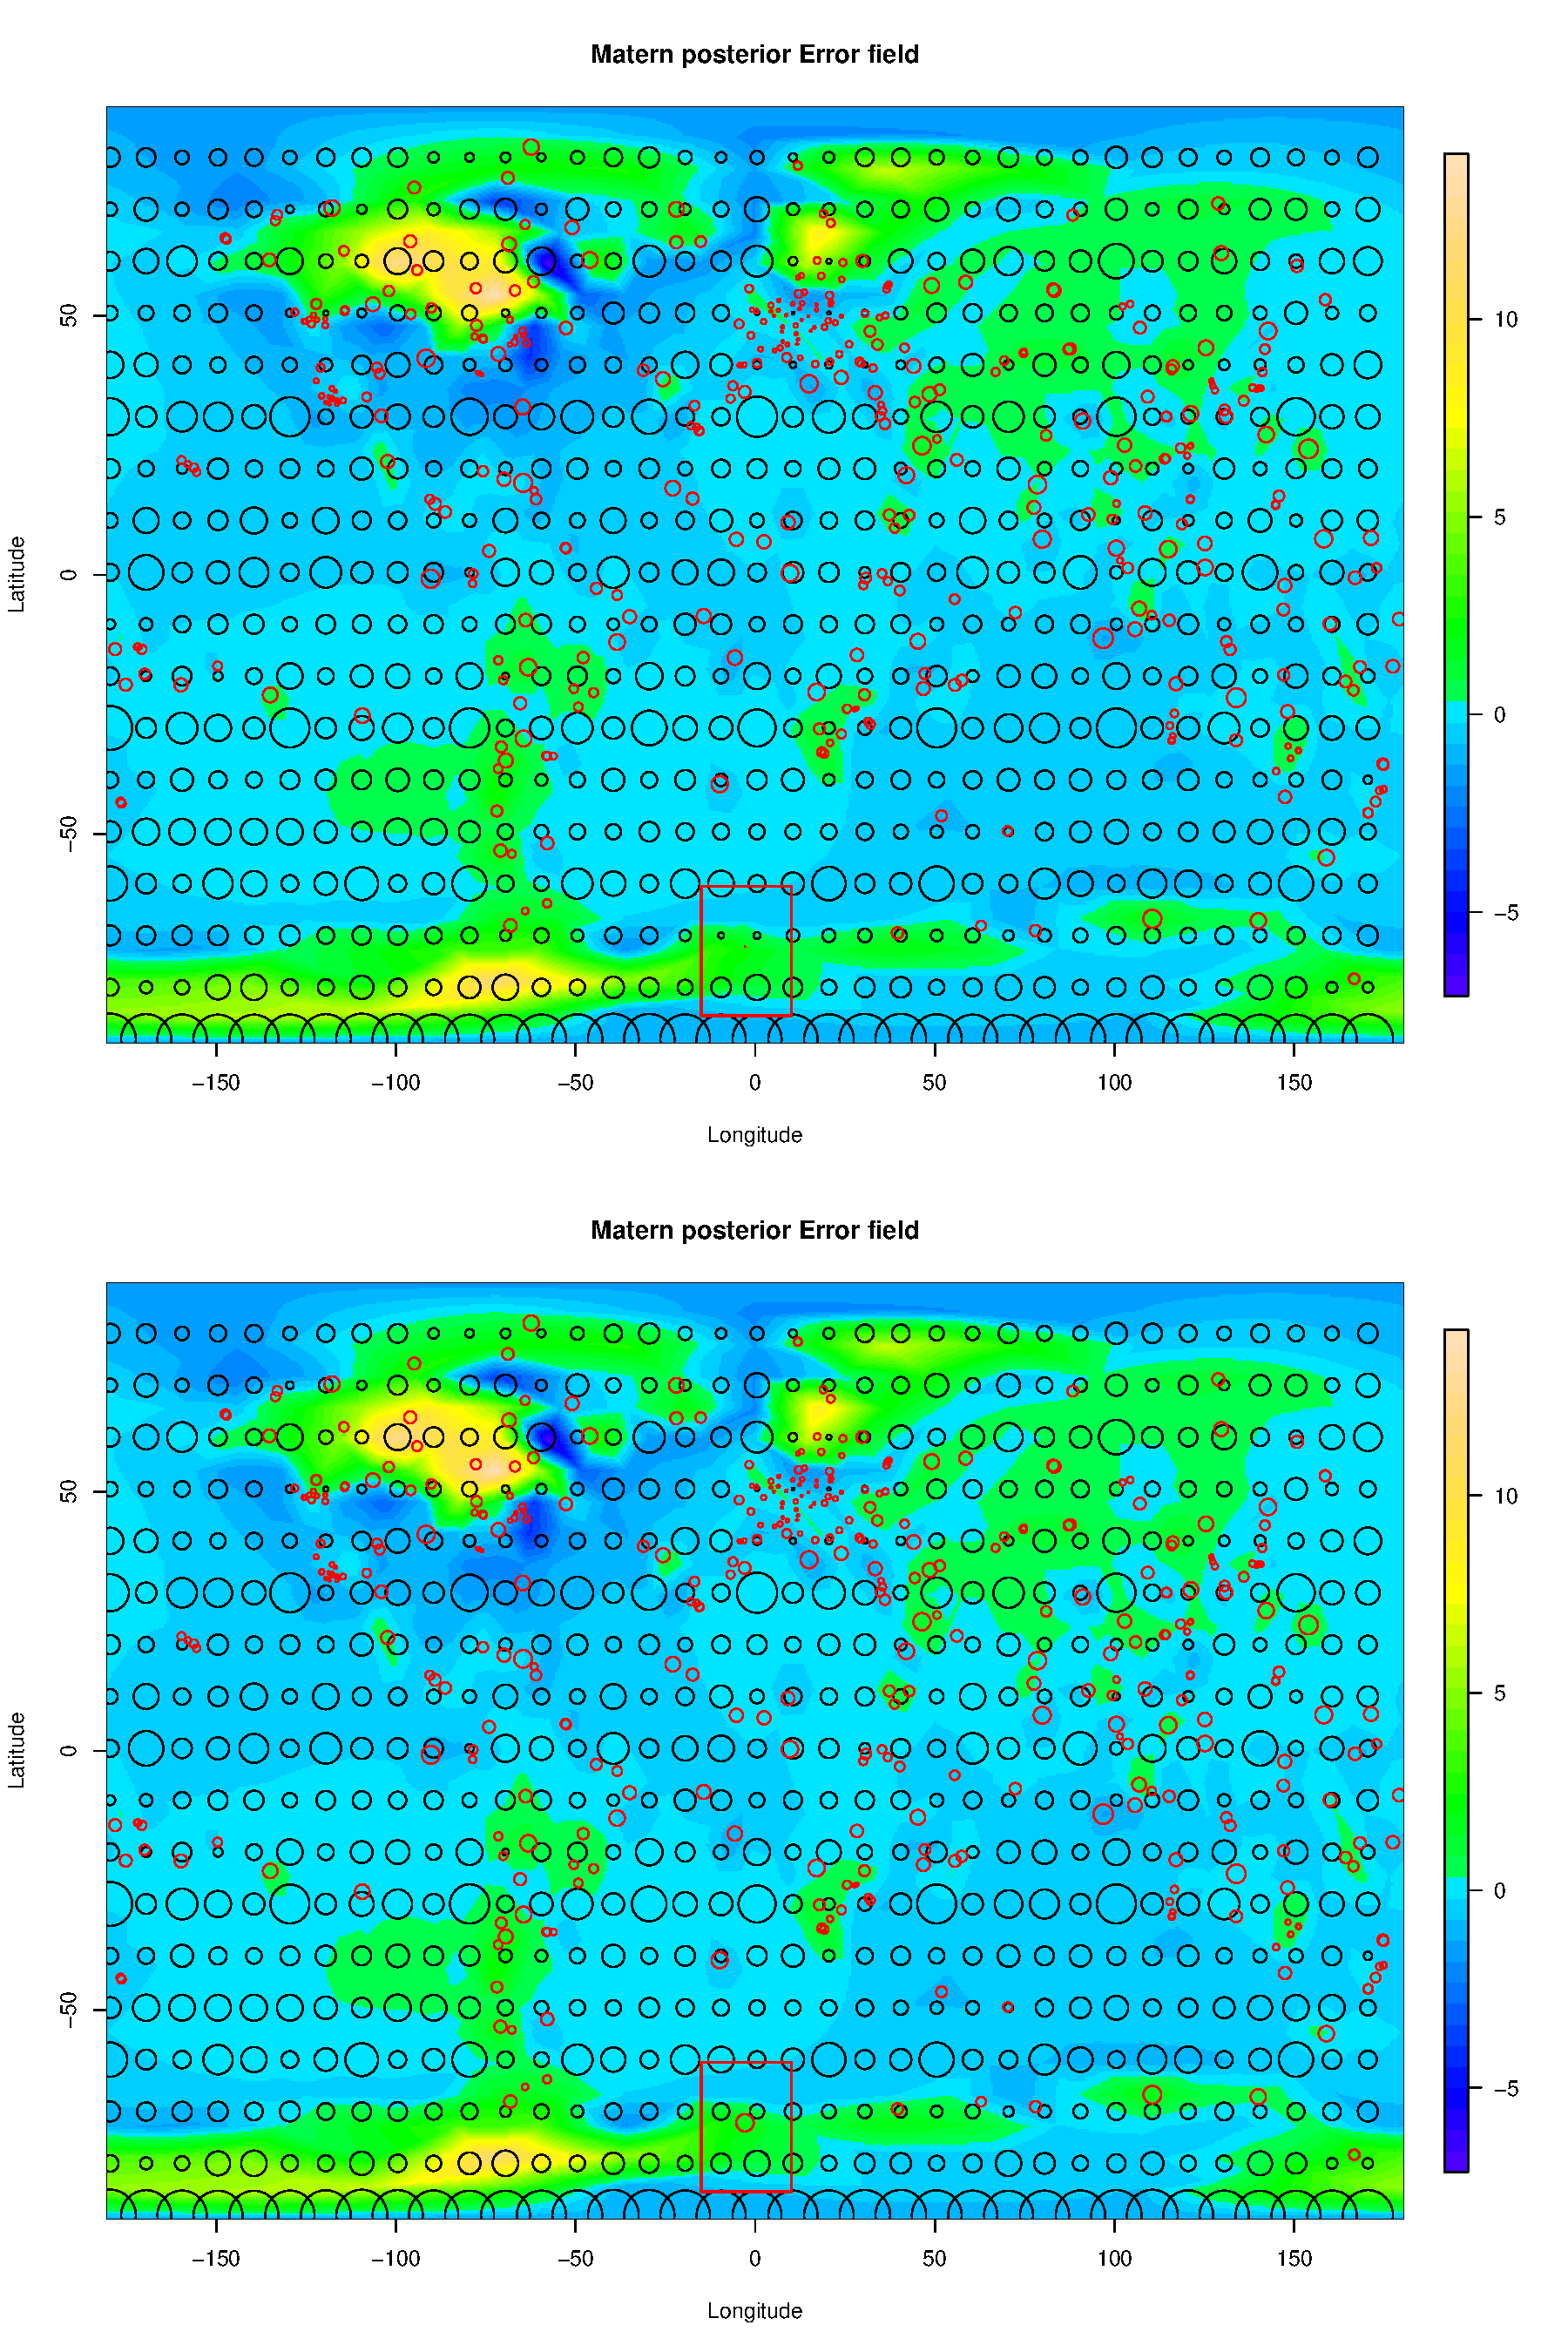
\includegraphics[scale=0.8]{fig/PointErr_GIAfield.pdf}
 \end{center}
 \caption[Posterior marginal standard errors of the latent field]{Posteriors marginal standard errors of the latent field using GPS data with different error on a single selected point. The selected point is marked as the circle within the red rectangle. Points are the GPS locations. Red points are positive errors and black negative. The circle size in the bottom plot represents the error size.}
 \label{fig:6}
 \end{figure}
 
 \subsection{Change error size in general}

 \begin{figure}[htbp]
 \begin{center}
 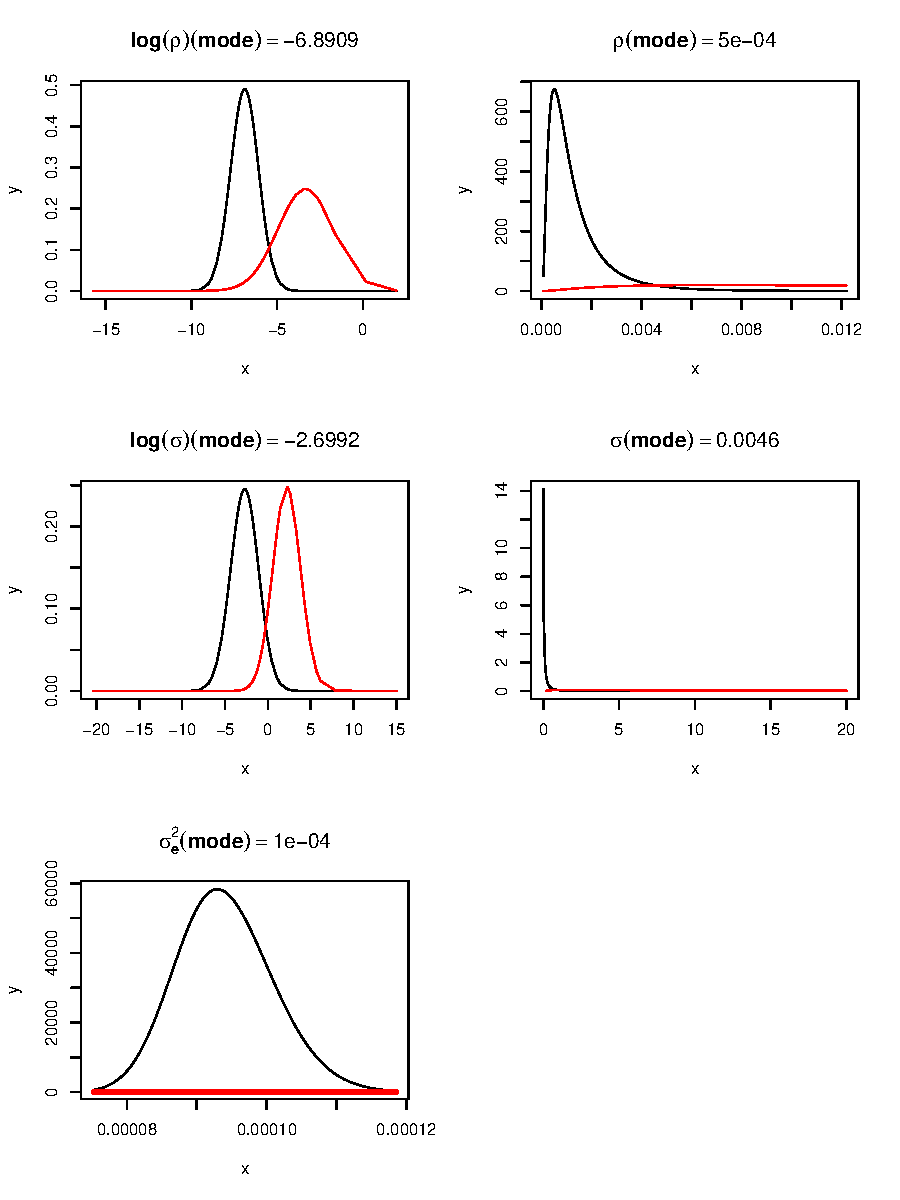
\includegraphics{fig/sMesh_sErr_hyperpar.pdf}
 \end{center}
 \caption[Hyper parameter with small errors]{Posteriors of hyper parameters using GPS data with small measurement errors. Black: posterior, Red: prior.}
 \label{fig:1}
 \end{figure}

\begin{figure}[htbp]
 \begin{center}
 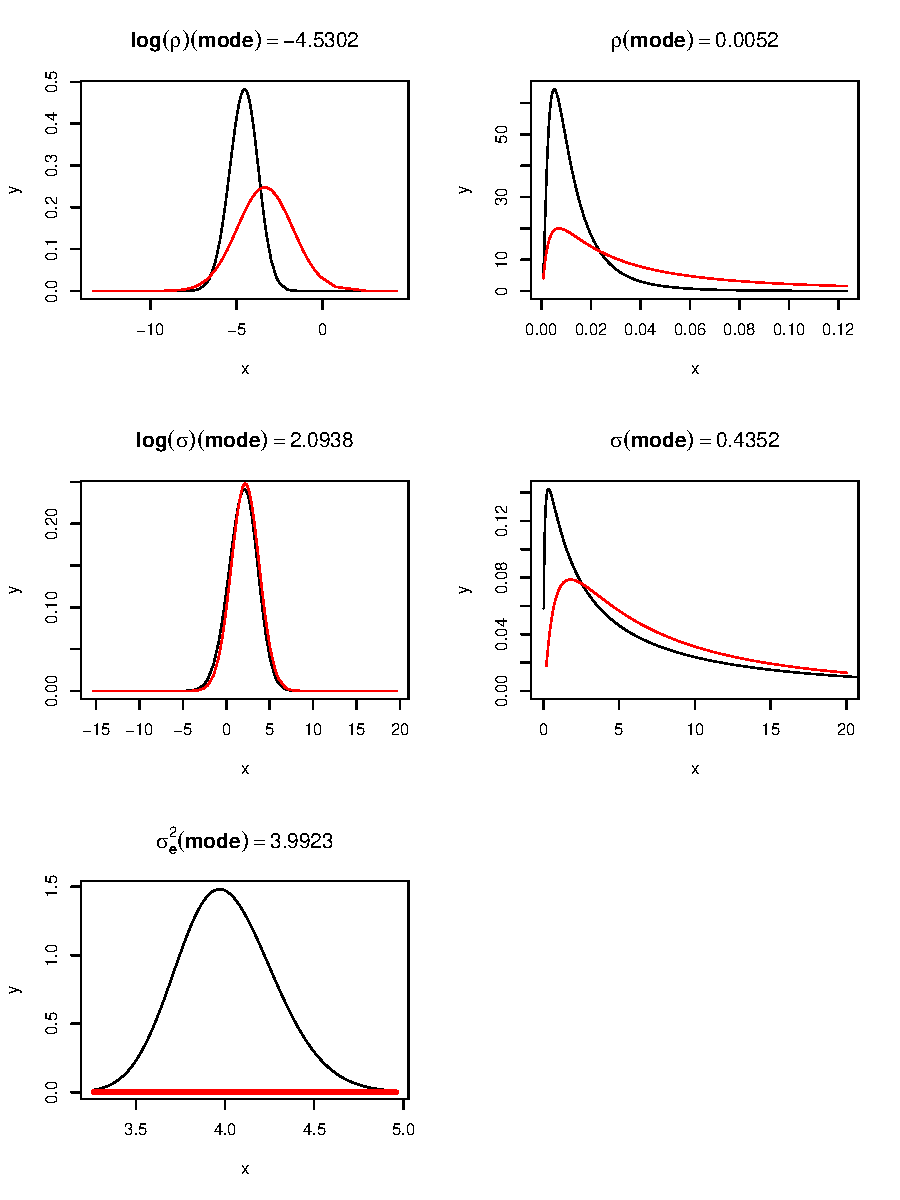
\includegraphics{fig/sMesh_LErr_hyperpar.pdf}
 \end{center}
 \caption[Hyper parameter with large errors]{Posteriors of hyper parameters using GPS data with large measurement errors. Black: posterior, Red: prior.}
 \label{fig:2}
 \end{figure}
 
  \begin{figure}[htbp]
 \begin{center}
 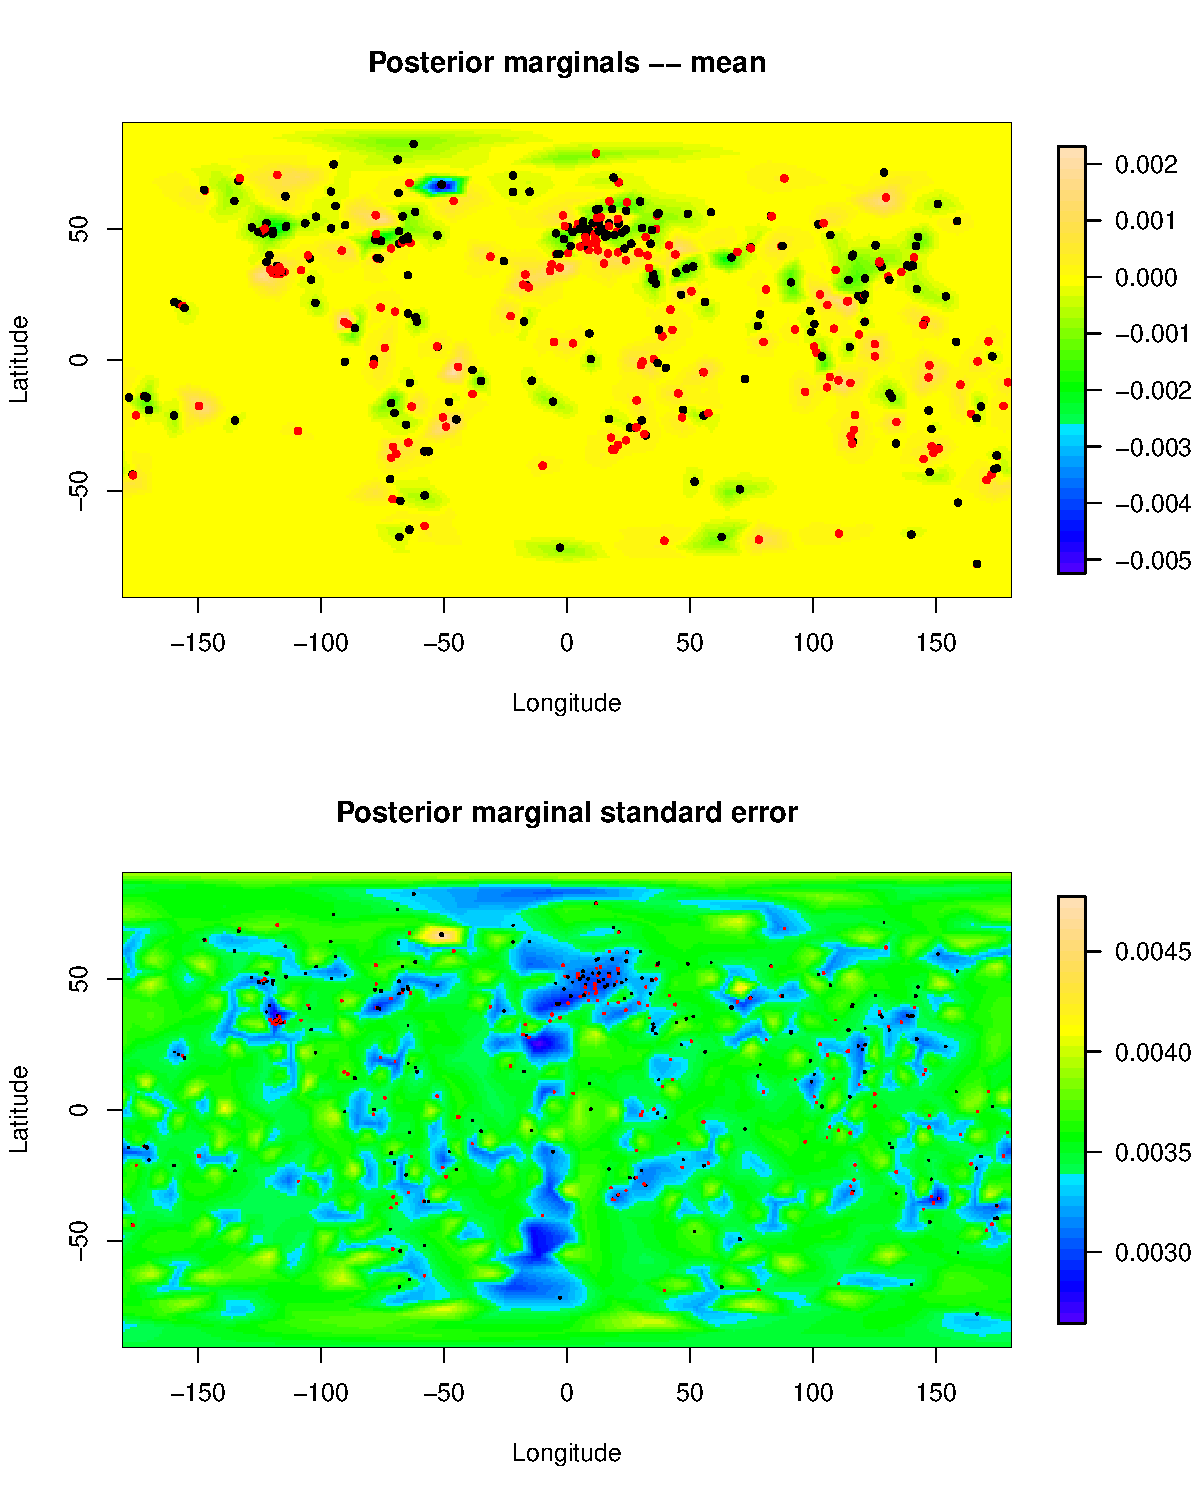
\includegraphics[scale=0.8]{fig/sMesh_sErr_GIAfield.pdf}
 \end{center}
 \caption[Posterior marginals of the latent field]{Posteriors marginal means and standard errors of the latent field using GPS data with small measurement errors. Points are the GPS locations. Red points are positive errors and black negative. The circle size in the bottom plot represents the error size.}
 \label{fig:3}
 \end{figure}
 
 \begin{figure}[htbp]
 \begin{center}
 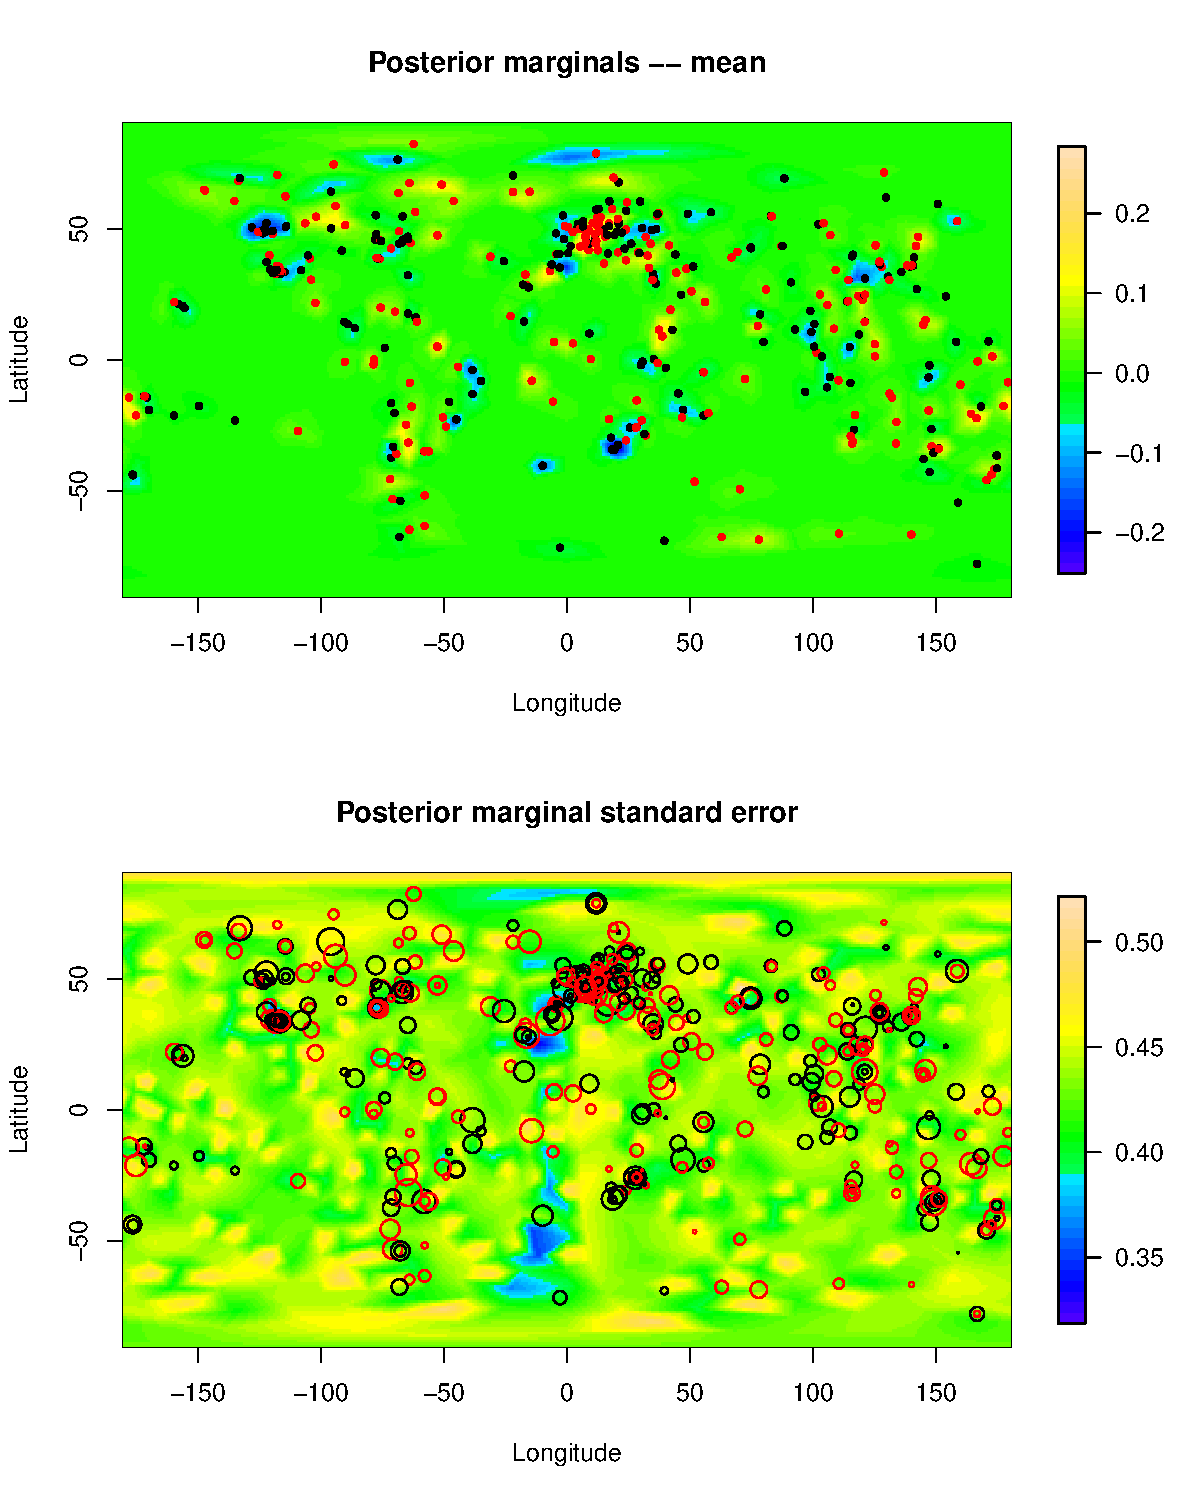
\includegraphics[scale=0.8]{fig/sMesh_LErr_GIAfield.pdf}
 \end{center}
 \caption[Posterior marginals of the latent field]{Posteriors marginal means and standard errors of the latent field using GPS data with large measurement errors. Points are the GPS locations. Red points are positive errors and black negative. The circle size in the bottom plot represents the error size.}
 \label{fig:4}
 \end{figure}
 
 
 
\section{Effect of Mesh size}

\begin{figure}[htbp]
 \begin{center}
 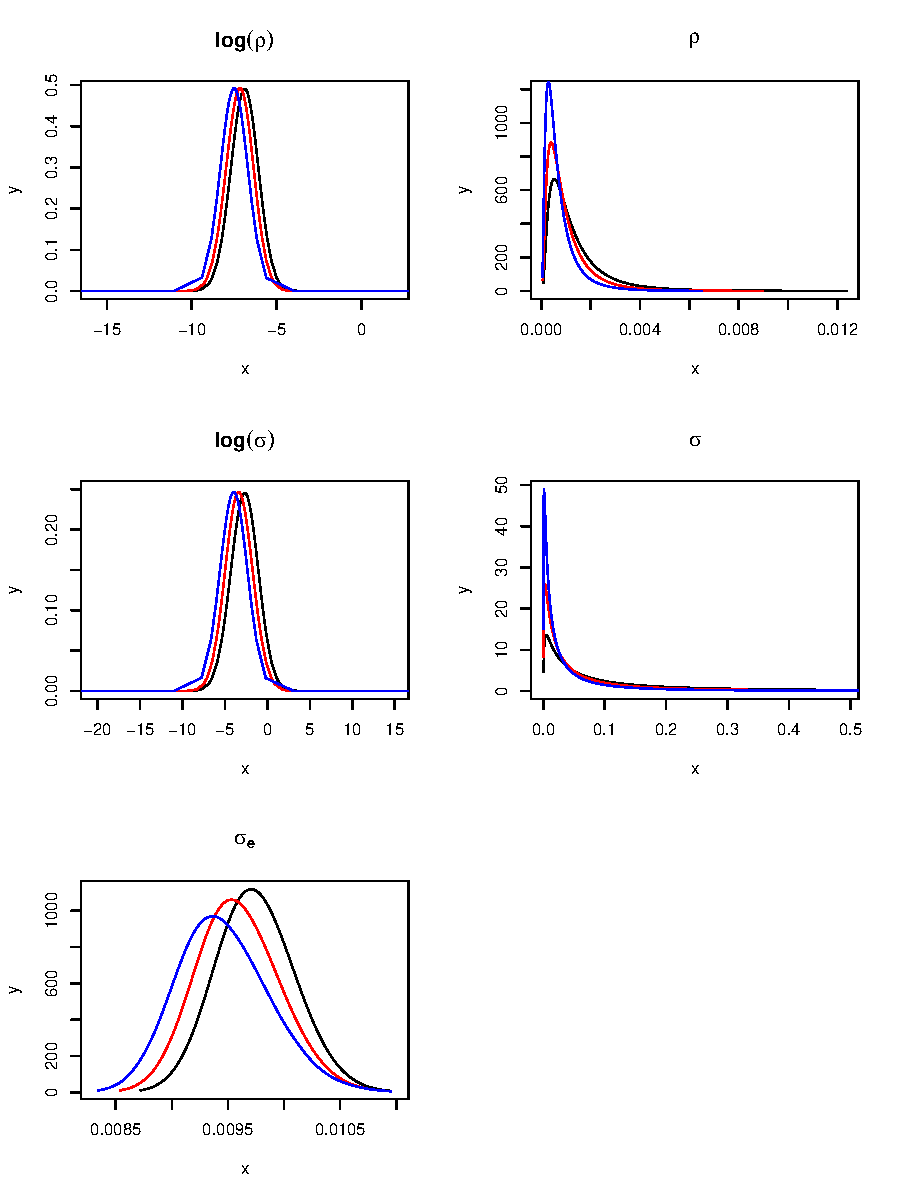
\includegraphics{fig/MeshSize_1hyperpar.pdf}
 \end{center}
 \caption[Hyper parameter for different mesh sizes]{Posteriors of hyper parameters estimated using different mesh sizes for the latnet process. Black: small, Red: medium, blue: large.}
 \label{fig:2}
 \end{figure}


 \begin{figure}[htbp]
 \begin{center}
 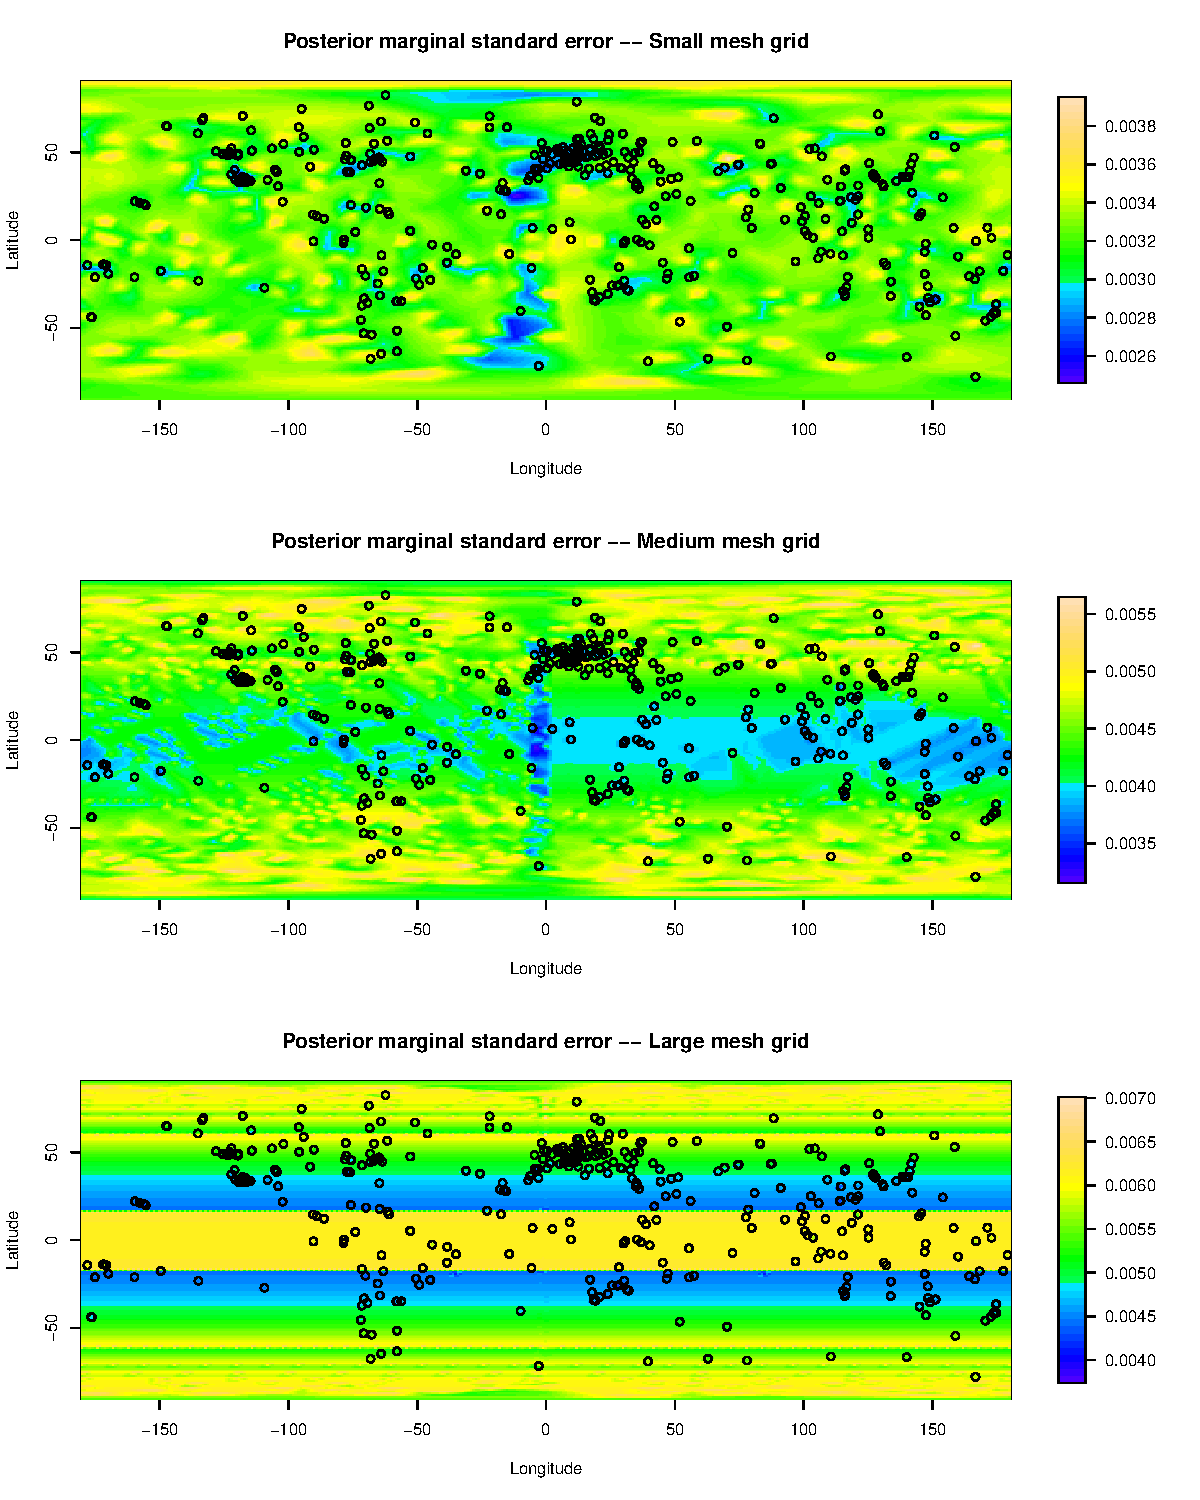
\includegraphics[scale=0.8]{fig/MeshSize_1GIAfield.pdf}
 \end{center}
 \caption[Posterior marginals of the latent field from different mesh size]{Posteriors marginal standard errors of the latent field with different mesh sizes. Points are the GPS locations.}
 \label{fig:4}
 \end{figure}
 














%------------Y(^_^) I'm the happy separation line (^_^)Y-------------%
\bibliographystyle{abbrvnat}
%\bibliography{references}




\end{document}